\chapter{Introduction}
Proteins are biological macromolecules that perform a large variety of functions in living cells comprising biochemical (enzymes), structural, mechanical, and signaling functions. They consist of chains composed of 20 different natural amino-acids called \underline{residues}, from 6 different families: positively (K, H, R) or negatively charged (E, D); polar neutral (S, N, Q, T); hydrophobic aromatic (F, W, Y); hydrophobic non-aromatic (A, V, I, L, M) and special cases (C, G, P). To perform their functions, proteins interact with small molecules referred to as ligands, which are able to bind to a protein with high affinity and specificity \cite{du2016insights}. These protein/ligand interactions are crucial in biology, particularly in the context of drug design \cite{li2019predicting}. Since proteins interact with a broad range of drugs, it is of particular interest to study their flexibility and the mechanisms of binding of ligands to proteins and its impact on the structural dynamics to gain insights into:
\vspace{-.25cm}
\begin{itemize}
	\item Phenomena involved in the biological processes and related to diseases \cite{silva2010ligand}
	\vspace{-.25cm}
	\item Discovery, design, and development of new drugs \cite{payandeh2021ligand}.
\end{itemize}
\vspace{-.25cm}
The atomic structural data provide key structural information of the ligand-bound and ligand-unbound (APO) proteins~\cite{chakraborti2021all}. \textbf{Nevertheless, the static information is not sufficient for understanding protein–ligand binding mechanisms, especially when pockets are highly flexible and contain several binding sites as it is the case for enzymes}. Therefore, molecular modeling and simulations at the atomic scale such as Molecular Dynamics (MD) or Normal Mode Analysis (NMA) are needed and are very powerful tools that provides a description of the dynamics and structures of protein–ligand systems with a high spatial and temporal resolution.

\section{3-D Structures of Proteins and the AlphaFold Revolution}

As explained above, proteins are essential biological macromolecules and the resolution of their three-dimensional (3-D) structure is crucial to understand their biological functions. For many years, considerable efforts have been made to resolve experimentally atomic structures of proteins using X-ray Diffrection (XRD), Nuclear Magnetic Resonance (NMR), or Cryo-Electron Microscopy (Cryo-EM). To date, around 200,000 3-D structuyres of proteins have been resolved experimentally and deposited in a database named Protein Data Bank (PDB, \url{https://www.rcsb.org}). However, it represents only a small fraction of resolved structures compared with the hundreds of billions of sequences of proteins referenced in the Universal Protein Resource (UniProt, \url{https://www.uniprot.org}) sequence database. This limitation is essentially due to the experimental constraints and exhaustive protocols that need to be performed to resolve such flexible structures, as presented in Table~\ref{TAB1}.

Therefore, being able to predict the 3-D structure of a protein from its sequence of amino acid, \textit{i.e.} the folding phenomenon, is very challenging. This has presented a formidable computational challenge for many decades. Two years ago, a significant advance was announced by DeepMind, a London-based Artificial Intelligence (AI) company now part of Google’s parent firm. They developed a AI program named AlphaFold\cite{AlphaFold} that was able to predict of protein 3-D structures with an accuracy competitive with experiments. Therefore, AlphaFold has the potential to revolutionize the way one consider the design of biosystems, allowing to predict 3-D structures of proteins that have not yet been experimentally characterized. This major breakthrough in the structural biology community will aid fundamental research for a better understanding of biological phenomena and for the development of new applications in medical or environmental research.

\begin{table}[h!]
	\begin{tabular}{cp{4cm}p{5cm}p{4.5cm}}
		\hline
		& Advantages & Disadvantages & Macromolecules\\
		\hline
		\multirow{4}{*}{XRD} & • Well developed & • Crystallization process & • Soluble proteins \\
		& • High resolution & • Diffraction process
		& • Proteins complexes \\
		& • Broad MW range & • Solid structure preferred & • Membranes, Ribosomes \\
		& • Model building &• Static crystalline structure & • DNA/RNA \\
		\hline
		\multirow{3}{*}{NMR} & • High resolution & • High sample purity & • MWs below 40–50 kDa \\
		& • Structure in solution & • Sample preparation & • Water soluble samples\\
		& • Dynamic study	& • Computational simulation & \\
		\hline
		\multirow{3}{*}{Cryo-EM} & • Sample preparation & • Relatively low resolution
		& • MWs > 150 kDa\\
		& • Native state & • Highly dependent on EM & • Large proteins\\
		& • Small sample size	& • EM equipment & • Complex compounds \\
		\hline
	\end{tabular}
	\caption{The comparison of X-ray crystallography, NMR and Cryo-EM. MW acrocym refers to molecular weight.}
	\label{TAB1}
\end{table}

\section{Glutathione Transferase}
Glutathione transferases (GSTs) belong to a ubiquitous superfamily of enzymes, which were originally discovered as detoxification enzymes, are one of the key enzymes involved in the metabolization of endogenous and exogenous molecules\cite{F-Neiers-GSTs}. GSTs are found in most living organisms, including insects and mammals. Xenobiotic molecules include chemicals naturally present in food sources as well as molecules produced industrially as pollutants and pesticides.

\begin{figure}[b!]
	\begin{minipage}{.59\textwidth}
		\textbf{(a)}\\
		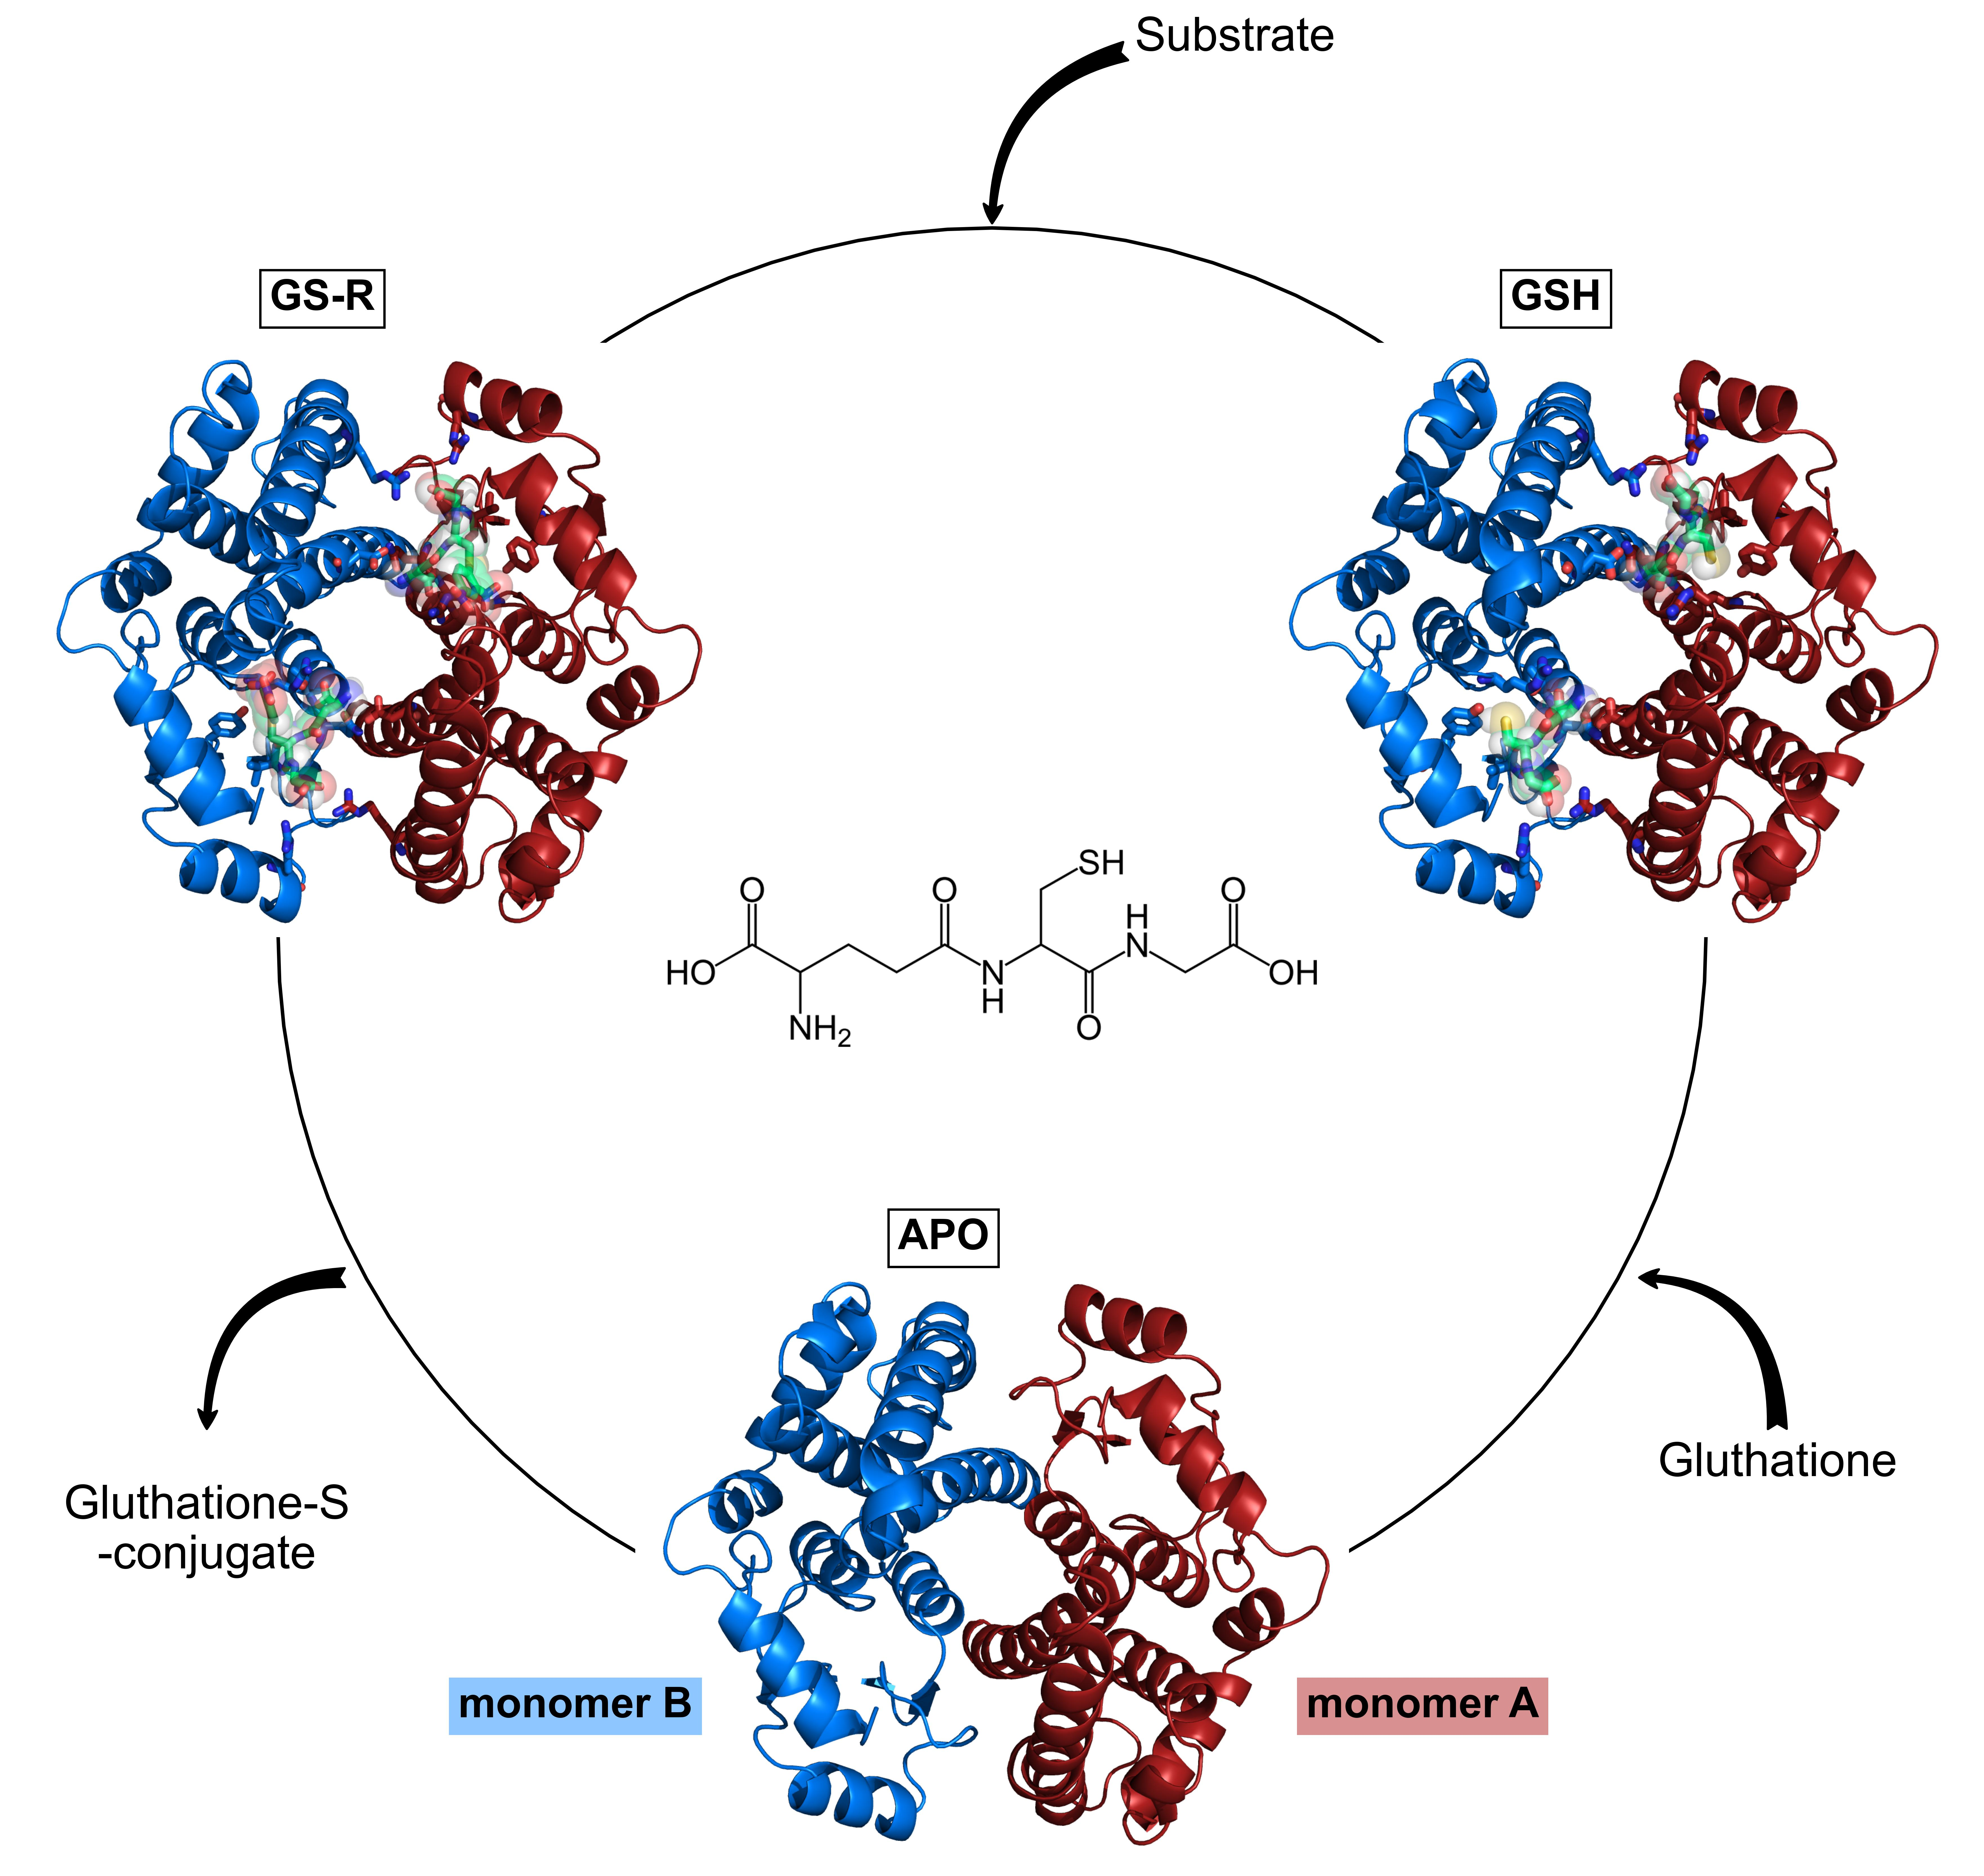
\includegraphics[width=.9\textwidth]{../figures/fig_1C_cycle.jpg}
	\end{minipage}
	\begin{minipage}{.4\textwidth}
		\textbf{(b)}\\
		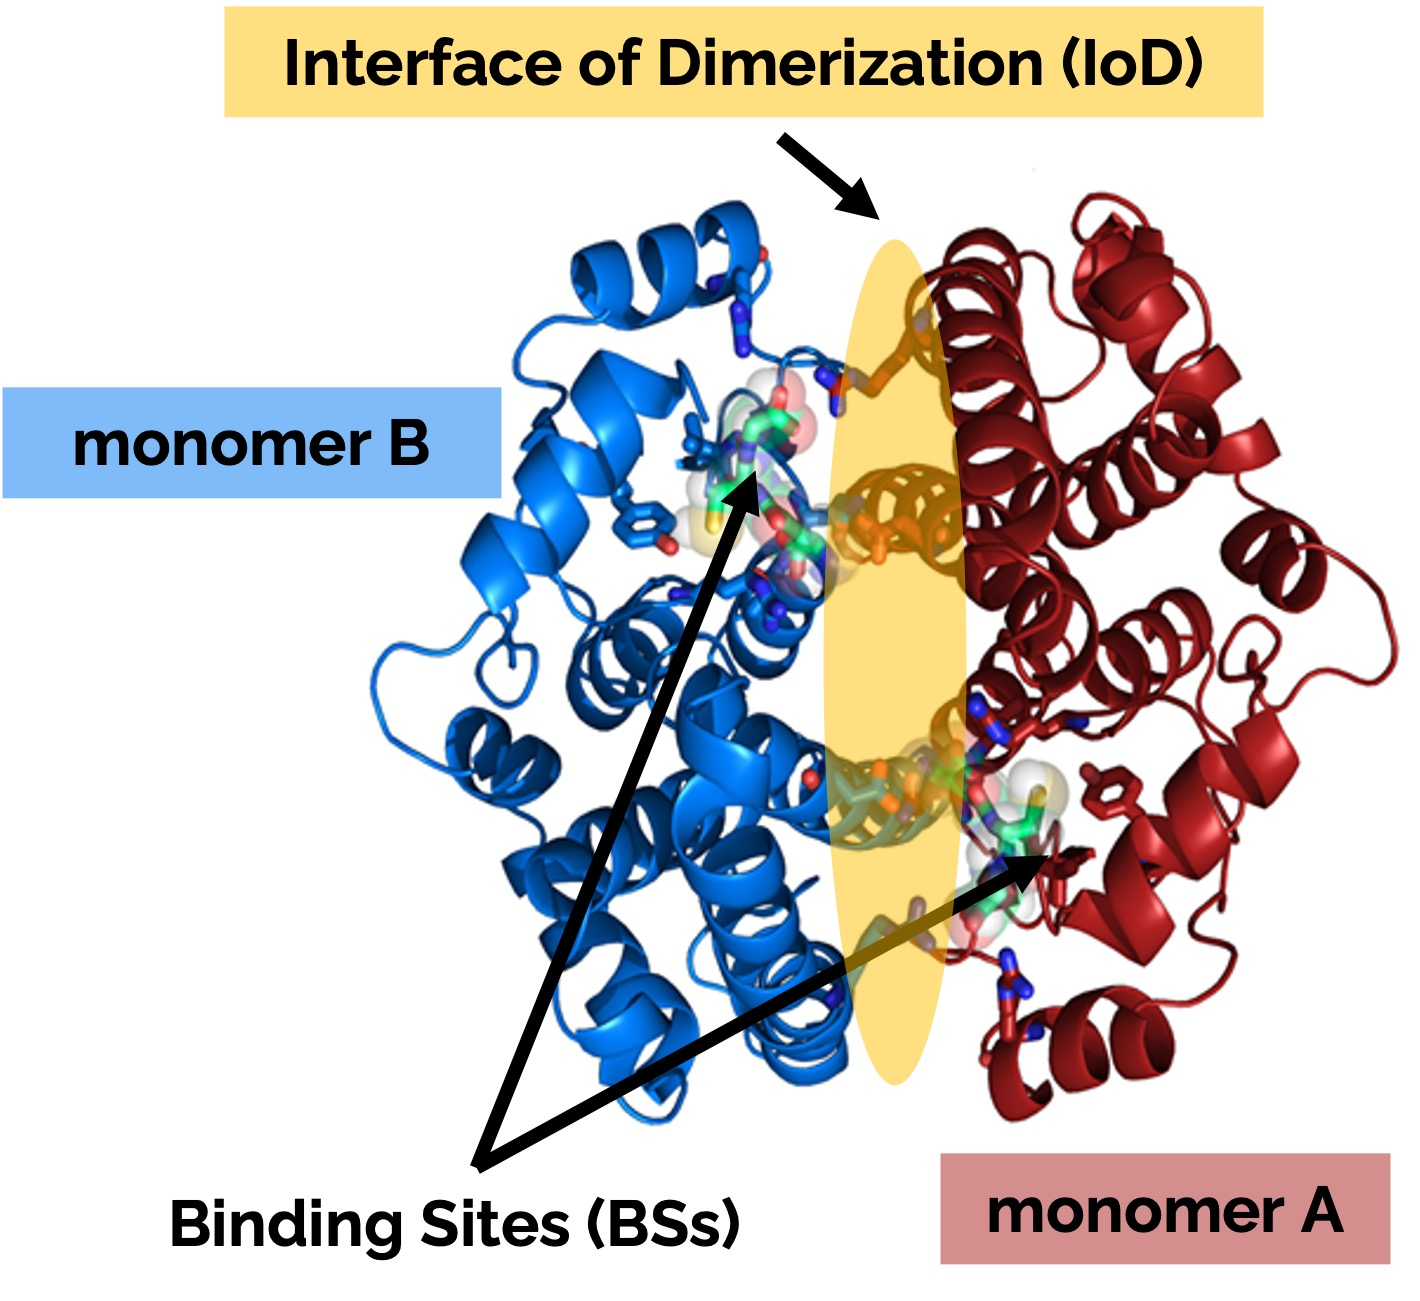
\includegraphics[width=1\textwidth]{../figures/fig_GST_BS_IoD.jpg}
	\end{minipage}
	\caption{(a). Catalytic cycle of GSH conjugation to electrophilic substrate. 3 forms of GSTA1 during the conjugation reaction cycle are highlighted: APO (no compound bound), GSH (Glutathione bound) and GS-R (Gluthatione-S-conjugated substrate). (b). Cartoon representation of GST dimer structures. Monomers A and B are shown in red and blue, respectively. Ligands are shown with green spheres.}
	\label{FIG2}
\end{figure}

GSTs metabolize a broad range of reactive toxic compounds by catalyzing the conjugation of reduced tripeptide glutathione ($\gamma$-Glu-Cys-Gly; named GSH) to the electrophilic center of a second substrate \cite{mannervik1985isoenzymes, armstrong1997structure, hayes2005glutathione} (FIg.~\ref{FIG2}a), the reactivity of GSH being due to the thiol group SH of the cysteine residue. The conjugation reaction occurs spontaneously but GST accelerates it dramatically. This process of detoxification protects cells against damages caused by both exogenous and endogenous molecules. GSTs were first discovered in liver cells \cite{combes1961liver}, and since then, they have been found to exhibit ligand-binding properties for a large variety of compounds, which are not always their enzymatic substrates \cite{axarli2004characterization}. Therefore, GSTs participate in diverse biological processes, making them multifunctional proteins. Moreover, GSTs are classified into three families according to their location in the cell: cytosolic, mitochondrial, and microsomal, which is not evolutively related to the two other classes \cite{oakley2011glutathione}. First-discovered and most-abundant cytosolic GSTs are divided into 13 classes based on homology of their sequences.Members of the same cytosolic class have at least $40\%$ of sequence identity, while members of different classes must have at most $25\%$ of sequence identity. 

With some exceptions, GSTs are catalytically active as dimers. GST monomers are, in general, made of 200 to 250 residues with a molecular weight generally comprised between 25 and 30 kDa~\cite{frova_glutathione_2006,board_glutathione_2013}. Each dimer structure contains two identical binding sites (BSs), with very important amino acids located at the interface of dimerization (IoD). These two structural features, \textit{i.e.} BSs and IoD are crucial for the biological function of GSTs and are of particular interest in the present work. In addition, these features are generally conserved among GST with some noticeable exceptions~\cite{board_glutathione_2013}. For instance, the residue of the BSs which interacts with the sulfur atom of GSH can be a Cysteine, a Serine, or a Tyrosin. And depending on the nature of this residue, GSTs develop slightly different catalytic functions and target a different range of substrates~\cite{mannervik_glutathione_1988,cummins_multiple_2011,deponte_glutathione_2013}. 

\section{Goal of the present work}

The goal of the present work is to develop a new methodology based on the AlphaFold program to predict the structural flexibility of an ensemble of GST enzymes, from static structures predicted by IA. The objective is to identify key residues related to the catalytic function of GSTs and their conservation in different classes of GST from a given organism. Therefore, the scientific question we would like to address is the following:

\vspace{.15cm}
\begin{tcolorbox}[width=\textwidth,colback={gray!20!white},title={\textbf{Scientific Question}},outer arc=0mm,colupper=black]    
	\centering
	\textbf{How the sequence of amino acid influence the structures and the flexibility of an ensemble of variants of GSTs from \textit{Drosophilia melanogaster} organism~?}
\end{tcolorbox}

In the present work, we focus our interest in GST enzymes from \textit{Drosophila melanogaster} organism (fruit fly), used as a model organism. Interactions between insects and plant’s chemicals lead to a major driving force in herbivorous insect evolution, hence this encourages the study of insect GSTs to understand how spontaneous mutations modify the stability, selectivity and the catalytic efficiencies of this enzyme family. For this organism, 42 GST structures have been identified\cite{F-Neiers-GSTs}, for which the $\delta$ and $\varepsilon$ classes are the largest ones 11 and 14 structures respectively. \textbf{This subset of 25 structures from $\delta$ and $\varepsilon$ classes is referred as the ensemble of GST structures considered in the present work.}

The methodology developed hereafter is summarized in Fig.~\ref{FIG3}. First, we performed Multiple Sequence Alignment (MSA) in order to compare the 25 amino acid sequences of the ensemble of GSTs and to estimate the percentage of identity existing between the sequences (see page X). Second, we predicted the 3-D atomic structures of the ensemble of 25 GSTs using the AlphaFold program considered here and compared them using structural analysis tools (see pages X). In addition, we predicted the position of an ensemble of ligands located in the binding sites of GST enzymes using the program AlphaFill (see page X). Fourth, from all the data generated using the previous tools, \textit{i.e.} MSA, AlphaFold and AlphFill, we studied the conservation of the residues involved in the binding sites and in the interface of dimerization of the ensemble of 25 GSTs that are crucial for their biological function in order to get insights into how the mutation of specific amino acids modified the characteristic of these GST structures. Last but not least, we studied the flexibility (Mean Square Fluctuations) of the ensemble of the 25 GST structures considered here using Normal Mode Analysis. Finally, we answer the scientific question given above by presenting the key amino acids involved in the structural dynamics of GSTs and their evolutionary conservation for the \textit{Drosophilia melanogaster} organism (see pages X).

\begin{figure}[h!]
	\footnotesize
	\begin{tikzpicture}[node distance=2cm,every text node part/.style={align=center}]
		\node (start) [startstop] {\textbf{1. SEQUENCES}};
		\node (startM) [decision, below of=start,yshift=-1cm] {Multiple \\Sequence\\Alignment\\(MSA)};
		\draw [arrow] (startM) -- (start);
		

		\node (in1) [startstop, right of=start,xshift=2cm] {\textbf{2. STRUCTURES}};	
		\draw [arrowT] (start) -- (in1);
		\node (in1M) [decision, below of=in1,yshift=-1cm] {AlphaFold
		\\AlphaFill\\(AF)};
		\draw [arrow] (in1M) -- (in1);
		
		\node (dec1) [startstop, right of=in1,xshift=2cm,yshift=1.5cm] {\textbf{3A. CONSERVATION}};
		\draw [arrowT] (in1) -- (dec1);
			\node (dec1M) [decision, above of=dec1,yshift=.5cm] {MSA			\\+\\AF};
		\draw [arrow] (dec1M) -- (dec1);
		
		\node (dec2) [startstop, right of=in1,xshift=2cm,yshift=-1cm] {\textbf{3B. DYNAMICS}};
		\draw [arrowT] (in1) -- (dec2);
		\node (dec2M) [decision, below of=dec2,yshift=-1cm] {Normal
			\\Mode\\Analysis\\(NMA)};
		\draw [arrow] (dec2M) -- (dec2);
		
		\node (dec3) [startstop2, right of=dec1,xshift=3cm,yshift=-1cm] {\textbf{4. IDENTIFICATION}\\ \textbf{OF KEY RESIDUES}};
		\draw [arrowT] (dec1) -- (dec3);
		\draw [arrowT] (dec2) -- (dec3);
		\node (dec3M) [decision2, below of=dec3,yshift=-1cm] {MSA
			\\+\\AF\\+\\NMA};
		\draw [arrow] (dec3M) -- (dec3);
		
	\end{tikzpicture}
	\caption{Diagram of the methodology developed in the present work. Rounded boxes indicate the triggered property and diamonds indicate the technique used.}
	\label{FIG3}
\end{figure}